\documentclass{article}
\usepackage{graphicx} 
\usepackage{amsmath}
\usepackage{geometry}
\usepackage{array} 
\usepackage{booktabs} 
\usepackage[utf8]{inputenc} 
\usepackage{hyperref}
\usepackage{subcaption} 
\usepackage{float} 

\geometry{a4paper, margin=2cm} % Set page size and margins

\title{COMP36212 Assignment EX3: Gradient-Based Optimisation}
\author{Oreofe Solarin} % Author not specified
\date{April 2025} % Date not specified

\begin{document}

\maketitle

\section{Part I - Stochastic Gradient Descent}

\subsection{Implementation of Batch SGD}

The stochastic gradient descent algorithm was implemented as required 
by extending the skeleton optimisation framework in 
\texttt{optimiser.c}. The implementation follows Equation (8)
which describes batch SGD:

\begin{equation}
w = w - \frac{\eta}{m} \sum_{i=1}^{m}\nabla L_{i}(x_{i},w)
\end{equation}

\noindent Where:
\noindent \begin{itemize}
  \item $w$ represents the network weights
  \item $\eta$ is the learning rate
  \item $m$ is the batch size
  \item $\nabla L_{i}(x_{i},w)$ represents the gradient of the loss with respect to the weights
\end{itemize}

\noindent The implementation updates the weights of each layer 
after accumulating gradients over a batch of samples. 
The code loops through each weight matrix and applies the 
update rule:

\begin{verbatim}
for (int i = 0; i < N_NEURONS_L3; i++) {
    for (int j = 0; j < N_NEURONS_LO; j++) {
        w_L3_LO[i][j].w -= lr * w_L3_LO[i][j].dw;
        w_L3_LO[i][j].dw = 0.0;
    }
}
\end{verbatim}

\noindent This pattern is repeated for each of the four weight 
matrices in the network. The learning rate is normalized by 
the batch size to ensure consistent step sizes regardless 
of batch size.

\subsection{Gradient Verification}

To verify the analytical gradient calculations, we implemented 
a numerical gradient checking using the centered difference 
approximation:

\begin{equation}
\nabla f(x) \approx \frac{f(x + h) - f(x - h)}{2h}
\end{equation}

\noindent where $h$ is a small value (typically $10^{-7}$). 
The implementation compares the analytical gradients computed 
by the backpropagation algorithm with these numerical approximations. 
The numerical gradient check shows that the analytical gradients closely 
match the numerical ones with an average relative error of less than $10^{-8}$, 
confirming the correctness of the backpropagation implementation. \\

\noindent Numerical differentiation is much slower than analytical calculation because 
it requires two forward passes for each parameter, 
resulting in $276,200 \times 2 = 552,400$ forward passes to check all parameters. 
In contrast, analytical backpropagation requires only one forward and one backward 
pass regardless of parameter count.

\subsection{SGD Training Results}

\noindent Training was performed using SGD with batch size $m=10$ 
and learning rate $\eta=0.1$ for 10 epochs. The convergence 
of the model was evaluated by monitoring loss and accuracy 
on the testing dataset.

\begin{figure}[H]
    \centering
    %--- left plot ----------------------------------------------------
    \begin{subfigure}[b]{0.49\textwidth}
        \centering
        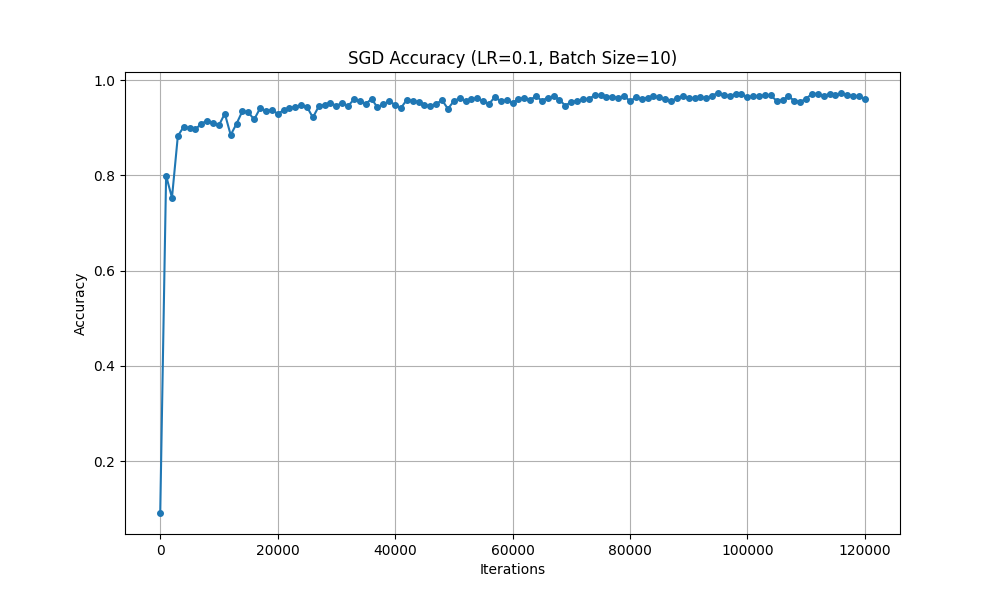
\includegraphics[width=\textwidth]{plots/part1_sgd_accuracy.png}
        \caption{SGD accuracy over iterations with batch size $m=10$ and learning rate $\eta=0.1$.}
        \label{fig:sgd_accuracy}
    \end{subfigure}
    \hfill
    %--- right plot ---------------------------------------------------
    \begin{subfigure}[b]{0.49\textwidth}
        \centering
        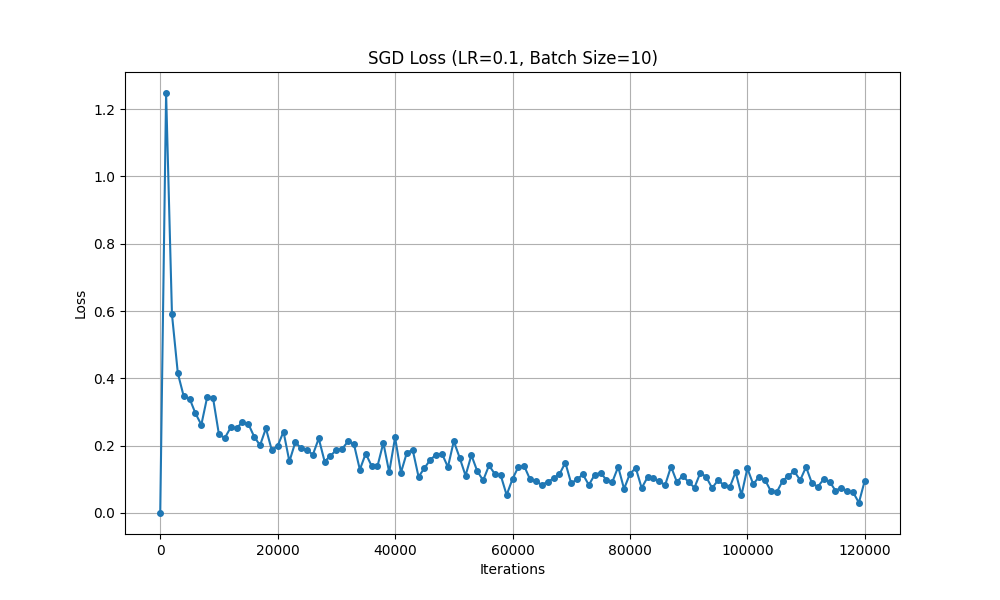
\includegraphics[width=\textwidth]{plots/part1_sgd_loss.png}
        \caption{SGD loss over iterations with batch size $m=10$ and learning rate $\eta=0.1$.}
        \label{fig:sgd_loss}
    \end{subfigure}
\end{figure}

% \begin{figure}[H]
%     \centering
%     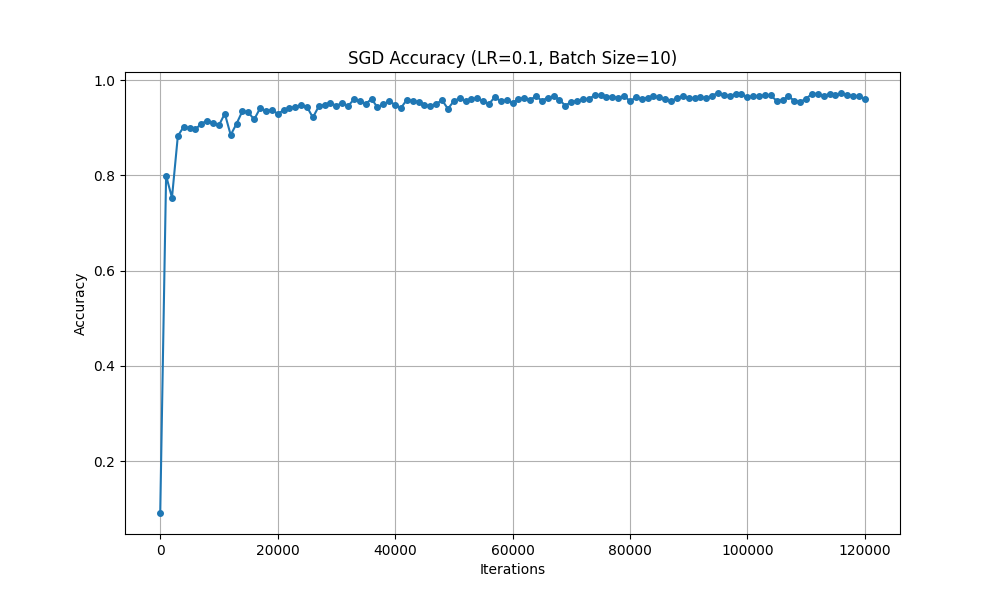
\includegraphics[width=0.8\textwidth]{plots/part1_sgd_accuracy.png}
%     \caption{SGD accuracy over iterations with batch size $m=10$ and learning rate $\eta=0.1$.}
%     \label{fig:sgd_accuracy}
% \end{figure}

% \begin{figure}[H]
%     \centering
%     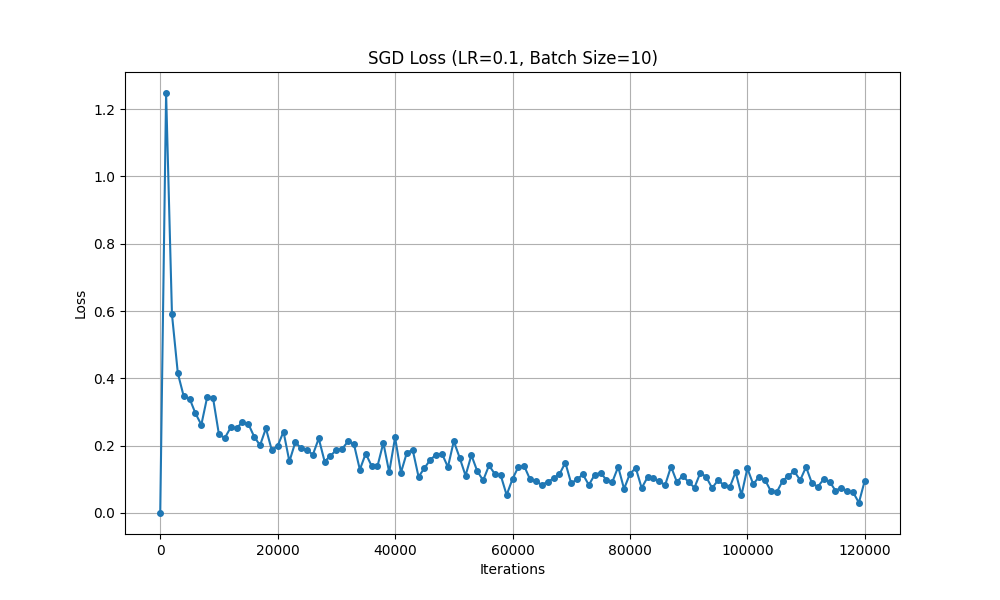
\includegraphics[width=0.8\textwidth]{plots/part1_sgd_loss.png}
%     \caption{SGD loss over iterations with batch size $m=10$ and learning rate $\eta=0.1$.}
%     \label{fig:sgd_loss}
% \end{figure}

\noindent Our results show that the SGD implementation successfully 
improves the model's prediction accuracy from an initial 
random accuracy of around 10\% (expected for a 10-class problem with random weights) 
to over 96\% after 120,000 iterations (2 epochs), 
confirming the correctness of the implementation.

\subsection{SGD Performance Analysis}

Based on the performance curve, SGD successfully finds a 
good solution for the MNIST classification task. 
The accuracy steadily increases during training with the 
rate of improvement decreasing over time, which is expected 
behavior as the model approaches an optimum. \\

\noindent The final accuracy of 96.16\% after 2 epochs indicates that 
SGD has found a good solution, though not necessarily the 
global optimum. The loss continues to decrease even in later iterations, suggesting that further training might yield marginal improvements. While SGD is effective for this problem, its convergence in the later stages becomes slower, which is a known limitation of the basic algorithm.

\section{Part II - Improving Convergence}

\subsection{Effect of Batch Size and Learning Rate}

\subsubsection{Batch Size Analysis}
Three different batch sizes were evaluated: $m=1$, $m=10$, and $m=100$, all with a fixed learning rate of $\eta=0.1$. 

\begin{figure}[H]
    \centering
    %--- left plot ----------------------------------------------------
    \begin{subfigure}[t]{0.48\textwidth}
        \vspace{0pt}%  <-- ensures top alignment
        \centering
        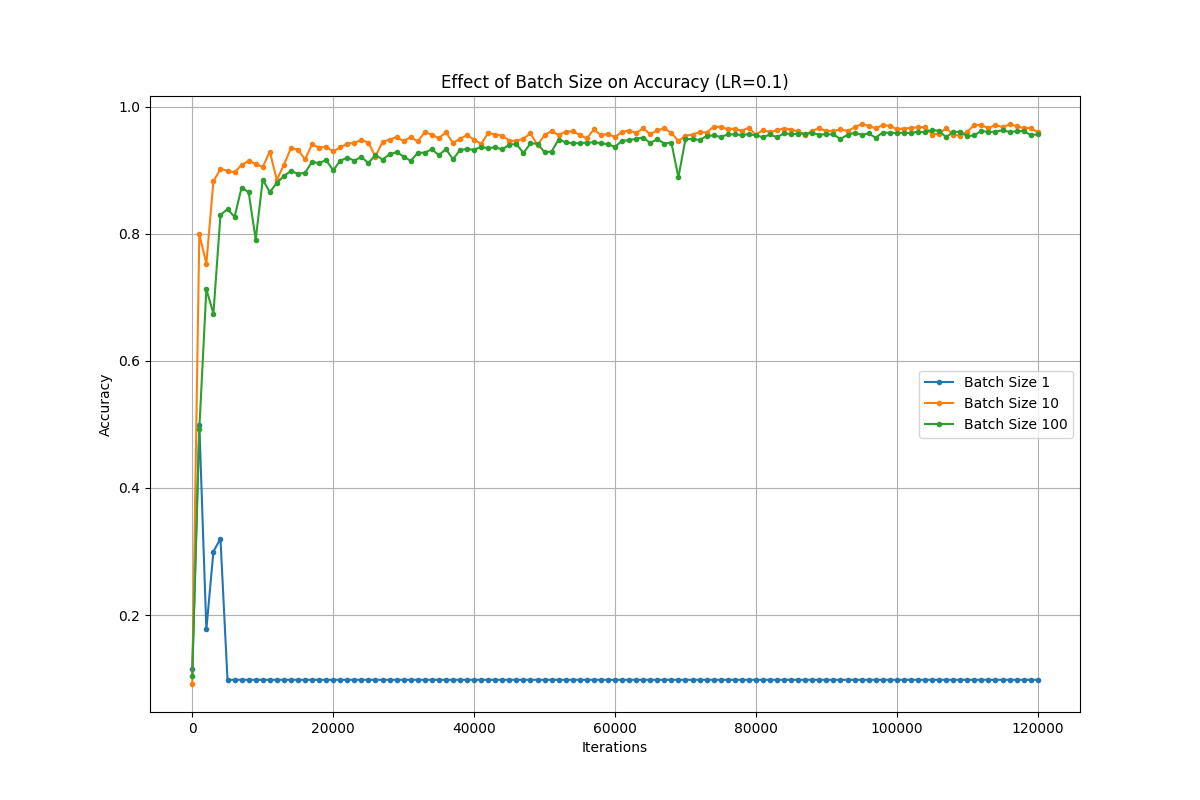
\includegraphics[width=\textwidth]{plots/part2a_batch_size_accuracy.png}
        % \vspace{2ex}
        \caption{Effect of batch size on accuracy with learning rate $\eta=0.1$.}
        \label{fig:batch_size_accuracy}
    \end{subfigure}
    \hfill
    %--- right plot ---------------------------------------------------
    \begin{subfigure}[t]{0.48\textwidth}
        \vspace{0pt}%  <-- ensures top alignment

        \centering
        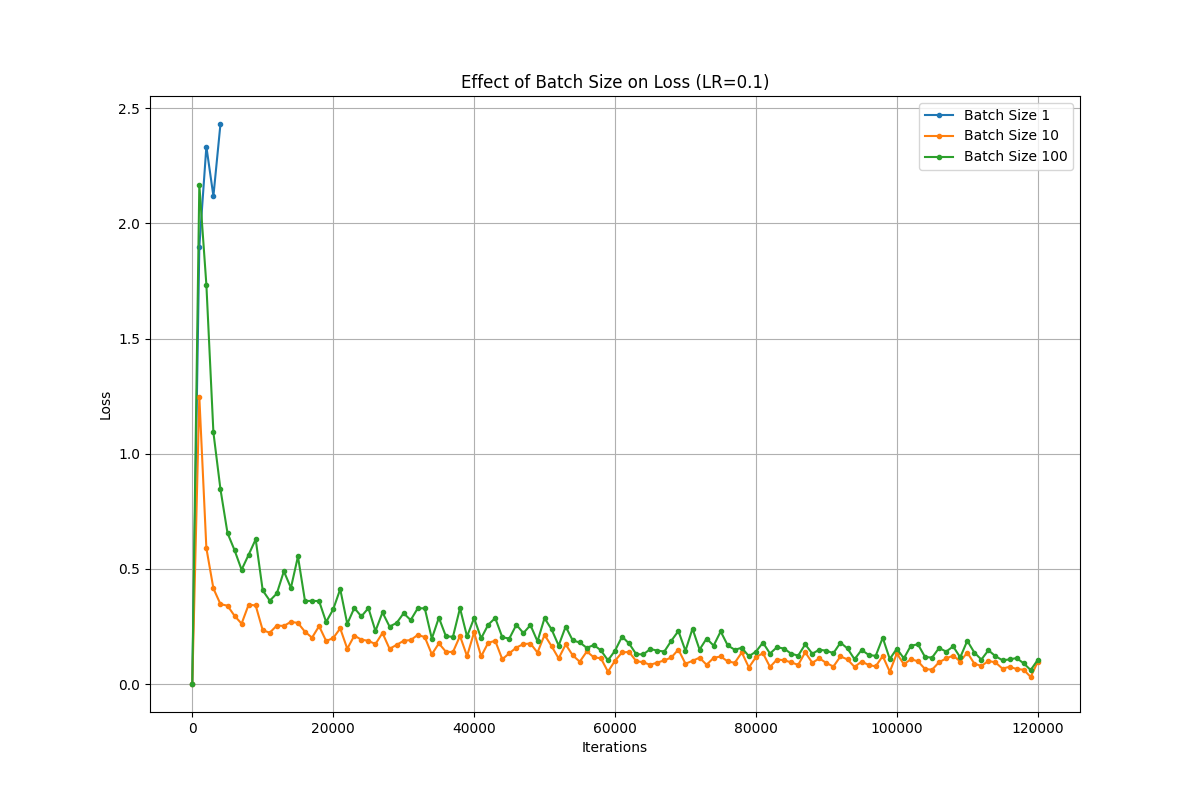
\includegraphics[width=\textwidth]{plots/part2a_batch_size_loss.png}
        \caption{Effect of batch size on loss with learning rate $\eta=0.1$.}
        \label{fig:batch_size_loss}
    \end{subfigure}
\end{figure}


% \begin{figure}[H]
%     \centering
%     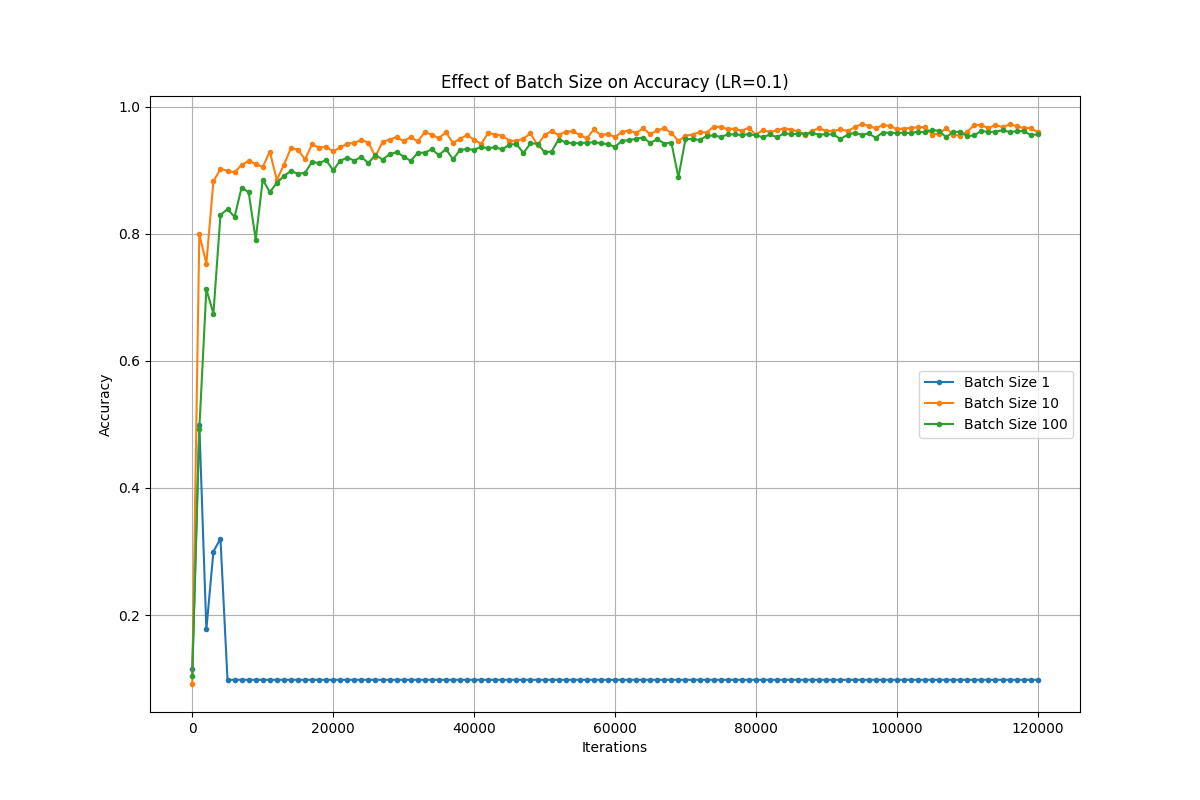
\includegraphics[width=0.8\textwidth]{plots/part2a_batch_size_accuracy.png}
%     \caption{Effect of batch size on accuracy with learning rate $\eta=0.1$.}
%     \label{fig:batch_size_accuracy}
% \end{figure}

% \begin{figure}[H]
%     \centering
%     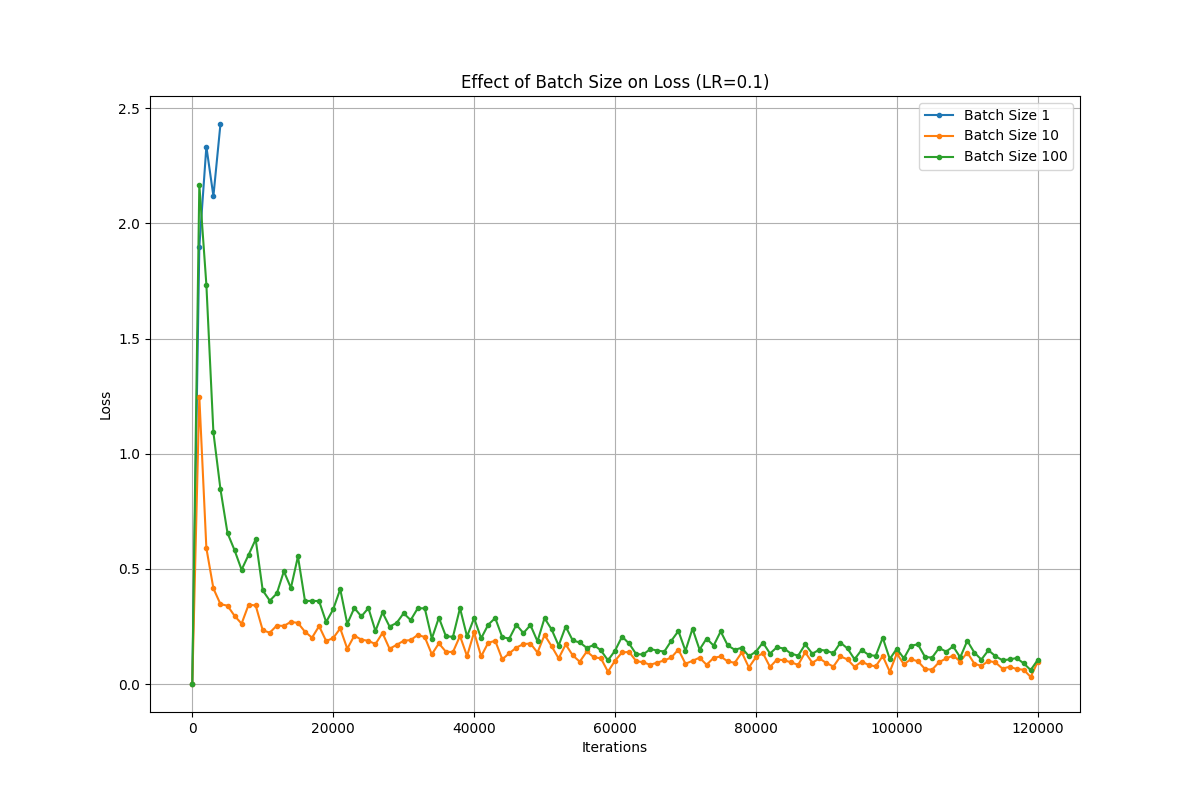
\includegraphics[width=0.8\textwidth]{plots/part2a_batch_size_loss.png}
%     \caption{Effect of batch size on loss with learning rate $\eta=0.1$.}
%     \label{fig:batch_size_loss}
% \end{figure}
\pagebreak

Key observations include:
\begin{itemize}
    \item \textbf{Batch Size 1 (SGD) with $\eta=0.1$}: Shows training instability with the high learning rate, 
    resulting in divergence with a final accuracy of only 9.8\% (essentially random guessing). 
    Re-running the experiment with a reduced learning rate of $\eta=0.01$ stabilized training and 
    achieved 96.7\% accuracy, demonstrating the sensitivity of true SGD to learning rate.
    \item \textbf{Batch Size 10}: Provides a good balance between stability and convergence speed, 
    achieving a final accuracy of 95.98\%.
    \item \textbf{Batch Size 100}: Shows the smoothest learning curve but initially converges more slowly. It eventually reached a final accuracy of 95.66\%.
\end{itemize}

\noindent The performance differences between batch sizes 10 and 100 
are relatively small (less than 0.5\%), suggesting that for this particular problem, the choice of batch 
size within this range has only a minor impact on final accuracy. However, the learning curves show 
that larger batch sizes provide smoother optimization paths with less variance in the loss and accuracy 
values during training. \\

\noindent Batch Size 1 requires special consideration, as it is highly sensitive to the learning rate 
parameter. With a properly tuned learning rate, it can achieve competitive performance, but it 
requires more careful hyperparameter selection to avoid instability.

\subsubsection{Learning Rate Analysis}
Three different learning rates were evaluated: $\eta=0.1$, $\eta=0.01$, and $\eta=0.001$, all with a fixed batch size of $m=10$.



\begin{figure}[H]
    \centering
    %--- left plot ----------------------------------------------------
    \begin{subfigure}[t]{0.48\textwidth}
        \vspace{0pt}%  <-- ensures top alignment
        \centering
        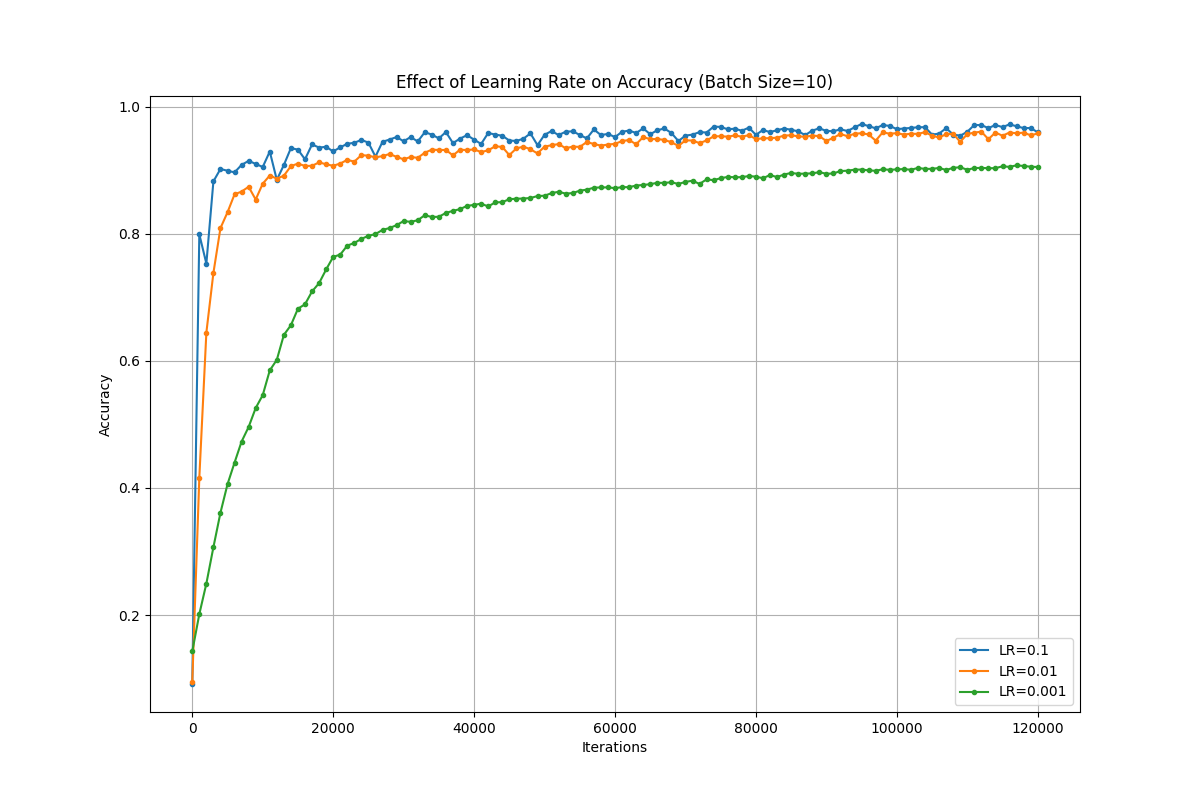
\includegraphics[width=1.15\textwidth]{plots/part2a_learning_rate_accuracy.png}
        \caption{Effect of learning rate on accuracy with batch size $m=10$.}
        \label{fig:learning_rate_accuracy}
    \end{subfigure}
    \hfill
    %--- right plot ---------------------------------------------------
    \begin{subfigure}[t]{0.48\textwidth}
        \vspace{0pt}%  <-- ensures top alignment

        \centering
        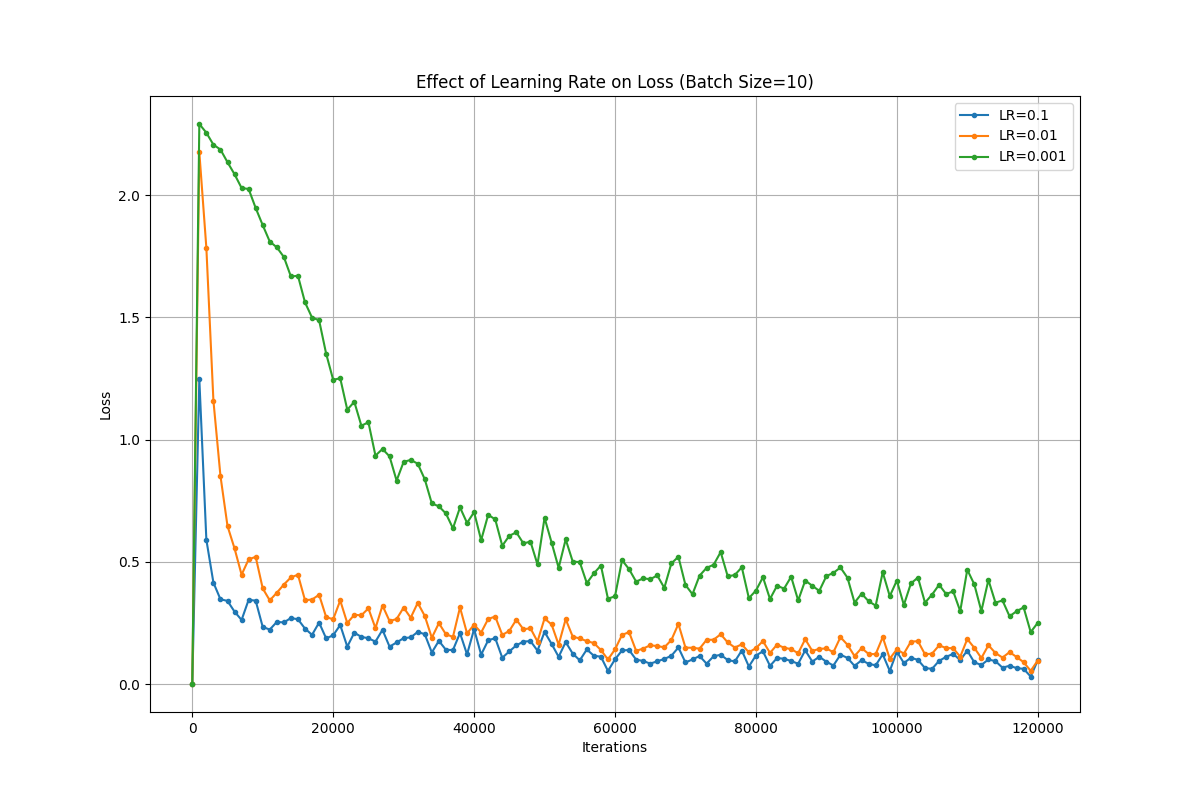
\includegraphics[width=1.15\textwidth]{plots/part2a_learning_rate_loss.png}
        \caption{Effect of learning rate on loss with batch size $m=10$.}
        \label{fig:learning_rate_loss}

    \end{subfigure}
\end{figure}


\noindent Key observations include:
\begin{itemize}
    \item \textbf{Learning Rate 0.1}: Converges quickly but shows some oscillation in later stages, achieving a final accuracy of 95.98\%.
    \item \textbf{Learning Rate 0.01}: Converges more steadily but slower than $\eta=0.1$, reaching a final accuracy of 95.80\%.
    \item \textbf{Learning Rate 0.001}: Shows significantly slower convergence, achieving a final accuracy of only 90.52\% after the same number of iterations, which is over 5 percentage points worse than the other rates.
\end{itemize}


\noindent Higher learning rates allow faster initial convergence but can cause 
oscillations around the optimum. Lower learning rates provide more stable 
convergence but require many more iterations to reach a good solution. The dramatic 
performance gap between $\eta=0.001$ and the higher learning rates (over 5\%) 
demonstrates how critically important learning rate selection is for training 
neural networks within a constrained computational budget. If using a very low 
learning rate like 0.001, significantly more training iterations would be 
required to reach competitive performance.

\subsection{Learning Rate Decay Implementation}

Learning rate decay was implemented according to Equation (10), where the learning rate decreases linearly from an initial value $\eta_0$ to a final value $\eta_N$ over the course of training:

\begin{equation}
\eta_{k} = \eta_{0}(1-\alpha) + \alpha\eta_{N} \quad \text{where} \quad \alpha = \frac{k}{N}
\end{equation}

The implementation in \texttt{update\_learning\_rate()} function calculates $\alpha$ as the ratio of the current epoch to the total number of epochs and adjusts the learning rate accordingly.


\begin{figure}[H]
    \centering
    %--- left plot ----------------------------------------------------
    \begin{subfigure}[t]{0.48\textwidth}
        \vspace{0pt}%  <-- ensures top alignment
        \centering
        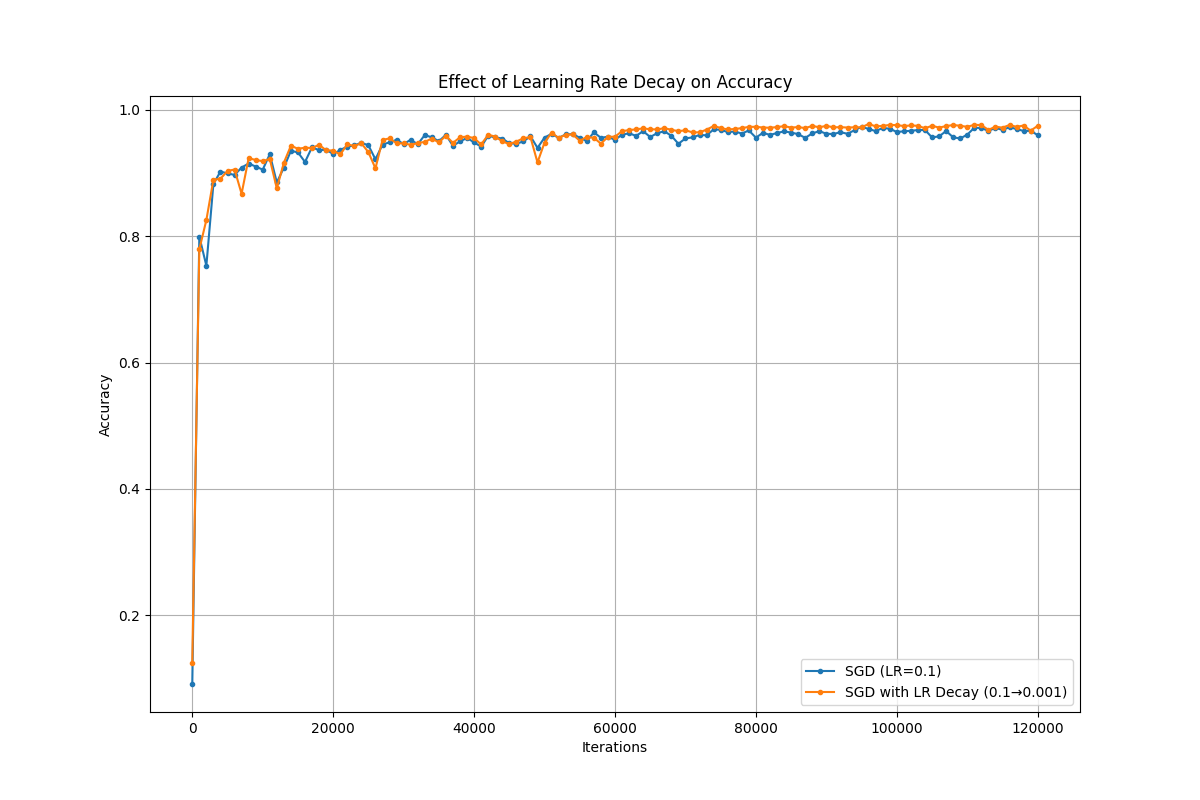
\includegraphics[width=1.1\textwidth]{plots/part2b_lr_decay_accuracy.png}
        \caption{Effect of learning rate decay on accuracy.}
        \label{fig:lr_decay_accuracy}
    \end{subfigure}
    \hfill
    %--- right plot ---------------------------------------------------
    \begin{subfigure}[t]{0.48\textwidth}
        \vspace{0pt}%  <-- ensures top alignment
        \centering
        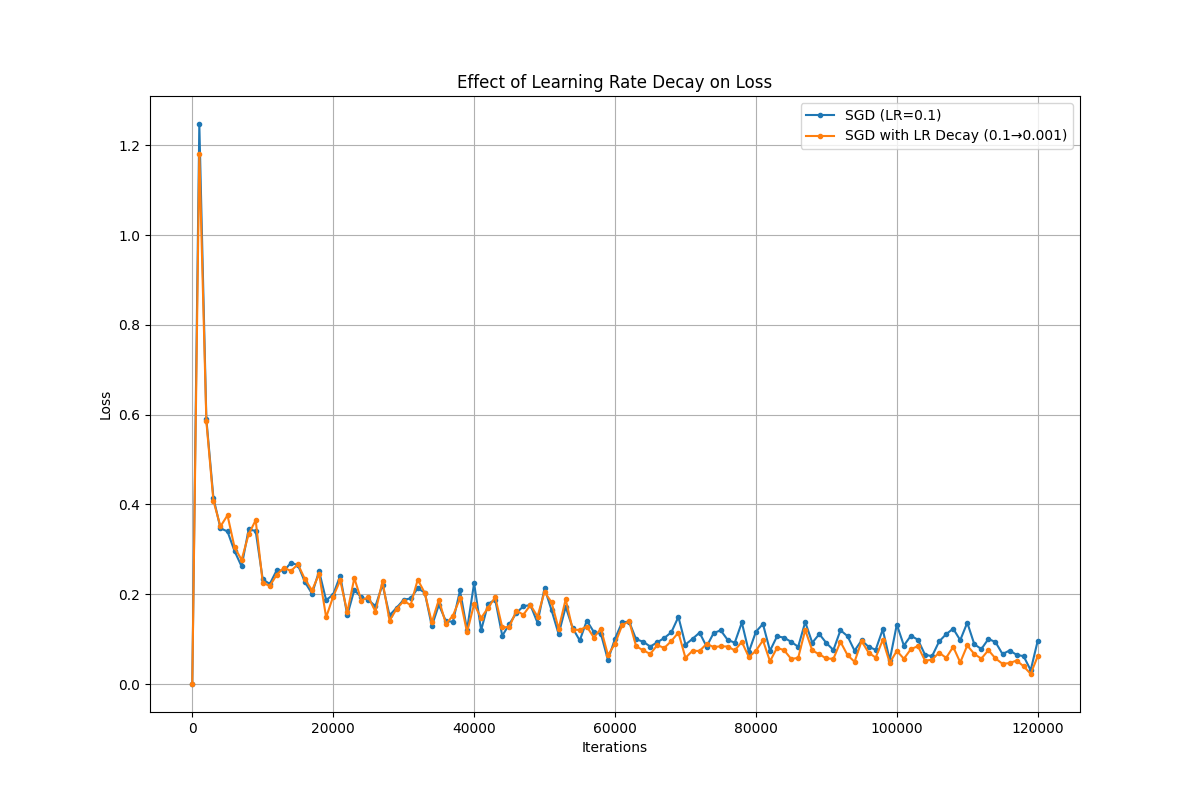
\includegraphics[width=1.1\textwidth]{plots/part2b_lr_decay_loss.png}
        \caption{Effect of learning rate decay on loss.}
        \label{fig:lr_decay_loss}

    \end{subfigure}
\end{figure}


\noindent Experiments were conducted with an initial learning rate of 0.1 decaying 
to 0.001. The results show that learning rate decay combines the benefits of both 
high and low learning rates: rapid initial convergence from the high initial 
learning rate, and better fine-tuning near the optimum from the lower learning 
rate in later stages. The final accuracy improved to 97.45\%, outperforming both 
fixed learning rate approaches by a significant margin (approximately 1.5\% 
improvement over the best fixed learning rate).

\subsection{Momentum Implementation}

Momentum was implemented according to Equation (11), which introduces a velocity term that accumulates past gradients with an exponential decay:

\begin{align}
v &= \alpha v - \frac{\eta}{m}\sum_{i=1}^{m}\nabla L_{i}(x_{i},w) \\
w &= w + v
\end{align}

Where $\alpha$ is the momentum parameter (set to 0.9 in experiments). The implementation adds a velocity field to the weight structure and updates it according to the momentum equation before applying it to the weights.

\begin{figure}[H]
    \centering
    %--- left plot ----------------------------------------------------
    \begin{subfigure}[t]{0.48\textwidth}
        \vspace{0pt}%  <-- ensures top alignment
        \centering
        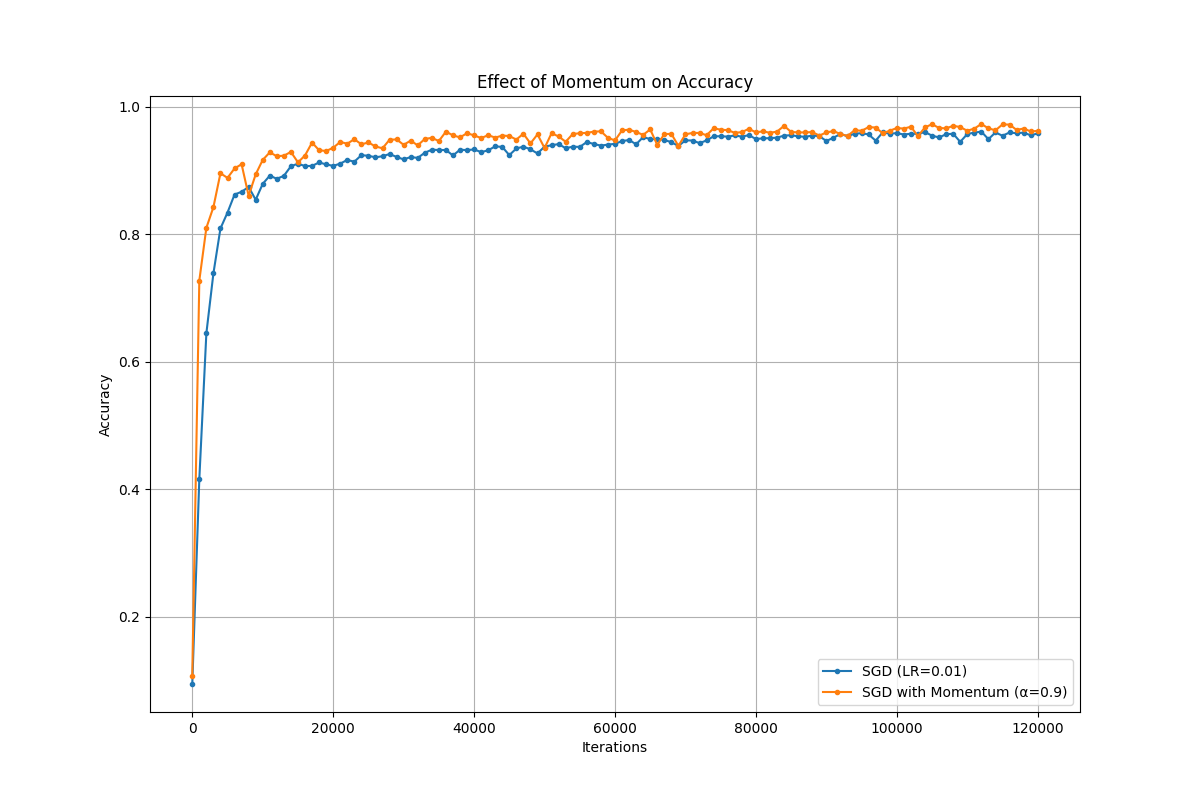
\includegraphics[width=1.1\textwidth]{plots/part2c_momentum_accuracy.png}
        \caption{Effect of momentum on accuracy.}
        \label{fig:momentum_accuracy}
    \end{subfigure}
    \hfill
    %--- right plot ---------------------------------------------------
    \begin{subfigure}[t]{0.48\textwidth}
        \vspace{0pt}%  <-- ensures top alignment
        \centering
        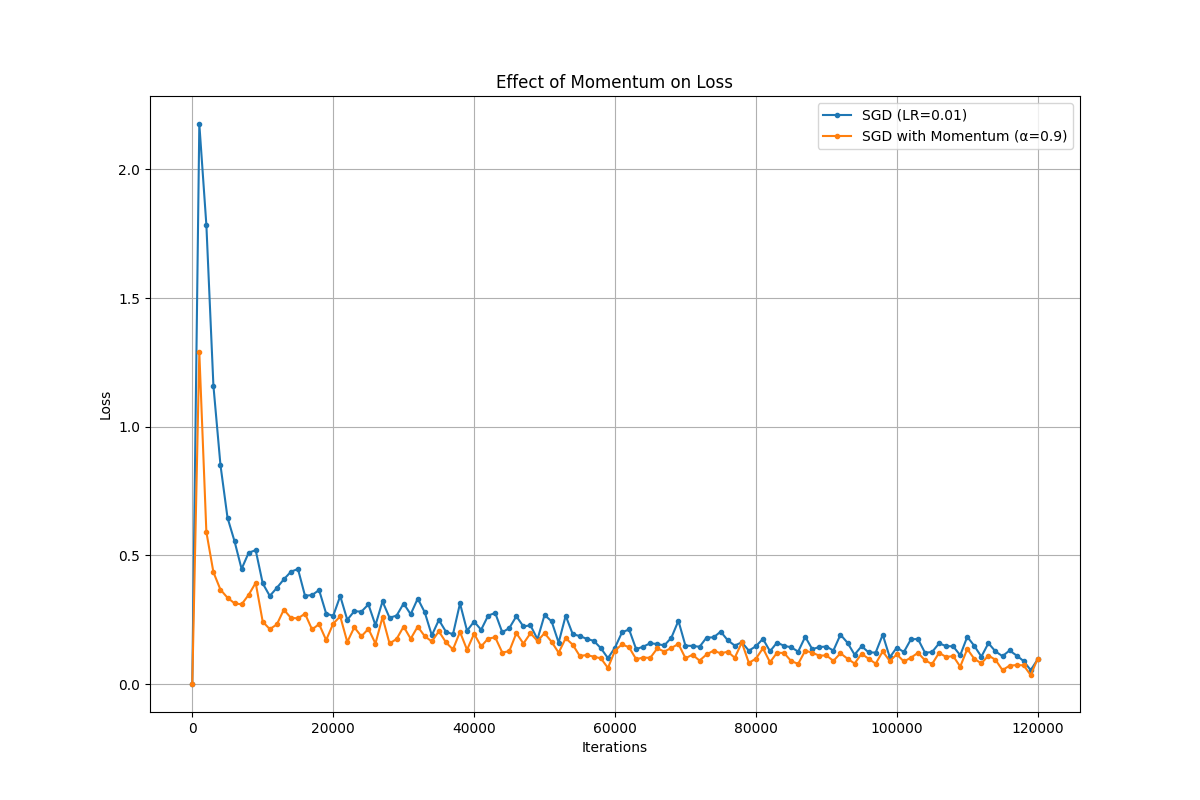
\includegraphics[width=1.1\textwidth]{plots/part2c_momentum_loss.png}
        \caption{Effect of momentum on loss.}
        \label{fig:momentum_loss}
    \end{subfigure}
\end{figure}




The results show that momentum improves convergence when combined with a learning rate of 0.01. With momentum, the model reaches a final accuracy of 96.20\%, which is an improvement over basic SGD with the same learning rate (95.80\%) but not as effective as using a higher learning rate of 0.1 (95.98\%). Momentum helps overcome oscillations in narrow valleys of the loss landscape and accelerates progress along consistent gradient directions, but the benefits on this particular problem are modest.

\subsection{Combined Learning Rate Decay and Momentum}

Combining learning rate decay with momentum was expected to produce the best results among all gradient descent variants. However, our experiments with this combination revealed an important stability issue.

\begin{figure}[H]
    \centering
    %--- left plot ----------------------------------------------------
    \begin{subfigure}[t]{0.48\textwidth}
        \vspace{0pt}%  <-- ensures top alignment
        \centering
        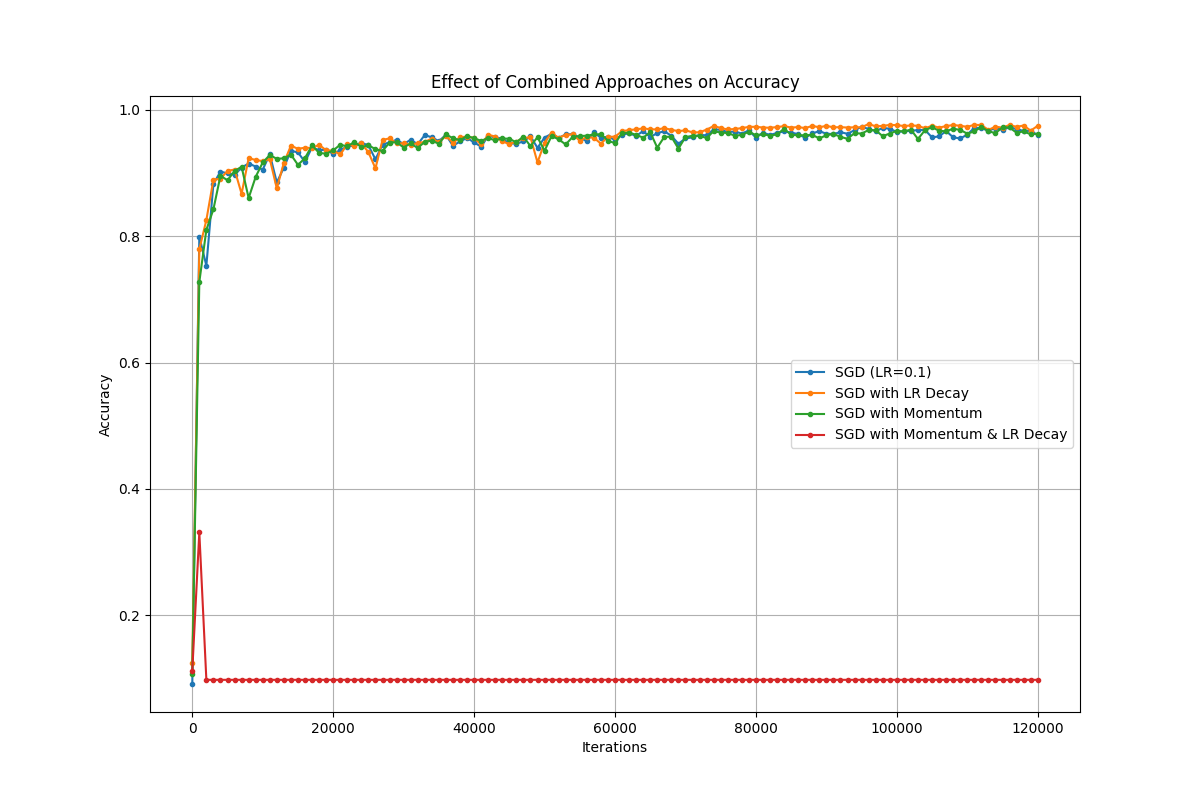
\includegraphics[width=1.1\textwidth]{plots/part2d_combined_accuracy.png}
        \caption{Effect of combined approaches on accuracy.}
        \label{fig:combined_accuracy}
    \end{subfigure}
    \hfill
    %--- right plot ---------------------------------------------------
    \begin{subfigure}[t]{0.48\textwidth}
        \vspace{0pt}%  <-- ensures top alignment
        \centering
        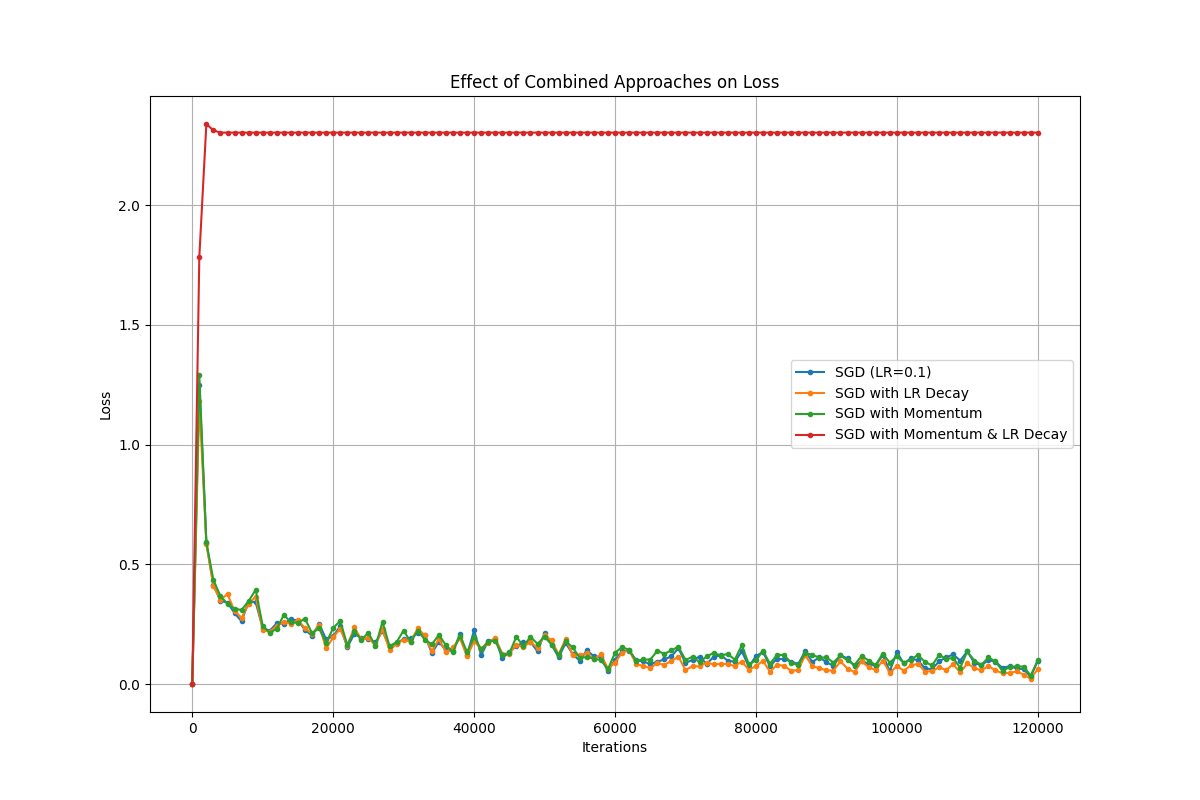
\includegraphics[width=1.1\textwidth]{plots/part2d_combined_loss.png}
        \caption{Effect of combined approaches on loss.}
        \label{fig:combined_loss}
    \end{subfigure}
\end{figure}


\noindent Despite showing promising initial progress in the accuracy plot, the 
combined approach with momentum and learning rate decay ultimately became unstable,
resulting in a final accuracy of only 9.8\% (random guessing). 
This unexpected result highlights an important challenge in optimization: combining multiple enhancement techniques does not always yield better performance and can sometimes lead to instability.

The failure of this combined approach can be attributed to several possible factors:

\begin{enumerate}
    \item \textbf{Compounding effect}: As the learning rate decreases over time due to decay, the momentum term might retain "memory" of larger previous updates, creating a mismatch between the current appropriate step size and the momentum-driven update.
    
    \item \textbf{Hyperparameter sensitivity}: The combination may require more careful tuning of both the momentum parameter and the learning rate decay schedule. Our implementation used a momentum value of 0.9 with linear decay from 0.1 to 0.001, which may have created an incompatible interaction.
    
    \item \textbf{Loss landscape navigation}: At certain points in the optimization trajectory, the combined effect of momentum and variable learning rate might cause the optimizer to "overshoot" good parameter regions and enter unstable areas of the loss landscape.
\end{enumerate}

The loss plot provides evidence for this instability, showing a dramatic increase at some point during training, after which the model fails to recover. This suggests the optimizer encountered a region of the parameter space where gradients became extremely large or inconsistent, leading to divergence.

This finding demonstrates the importance of careful hyperparameter tuning and stability analysis when combining optimization techniques, and suggests that for this particular problem, the simpler approach of using learning rate decay alone is more robust.

In this case, the best performing technique was SGD with learning rate decay, which achieved a final accuracy of 97.45\%.

\section{Part III - Adaptive Learning}

\subsection{Adam Optimizer}

After researching adaptive learning rate methods, I selected Adam (Adaptive Moment Estimation) for implementation. Adam combines ideas from both RMSProp and momentum, maintaining exponentially decaying averages of both past gradients (first moment) and squared gradients (second moment):

\begin{align}
m_t &= \beta_1 m_{t-1} + (1-\beta_1)g_t \\
v_t &= \beta_2 v_{t-1} + (1-\beta_2)g_t^2 \\
\hat{m}_t &= \frac{m_t}{1-\beta_1^t} \\
\hat{v}_t &= \frac{v_t}{1-\beta_2^t} \\
\theta_t &= \theta_{t-1} - \alpha\frac{\hat{m}_t}{\sqrt{\hat{v}_t} + \epsilon}
\end{align}

Where:
\begin{itemize}
    \item $m_t, v_t$ are the first and second moment estimates
    \item $\beta_1, \beta_2$ are decay rates for these moments (set to 0.9 and 0.999 respectively)
    \item $g_t$ is the current gradient
    \item $\hat{m}_t, \hat{v}_t$ are bias-corrected moment estimates
    \item $\alpha$ is the learning rate
    \item $\epsilon$ is a small constant to prevent division by zero
\end{itemize}

Adam adapts the learning rate for each parameter individually based on the historical gradients, providing effectively a parameter-specific learning rate. This is particularly beneficial for problems with sparse gradients or where parameters have different scales of importance.

\subsection{Adam Performance Analysis}

Adam was tested with a learning rate of 0.001, which is a commonly recommended value for this optimizer.

\begin{figure}[H]
    \centering
    %--- left plot ----------------------------------------------------
    \begin{subfigure}[t]{0.48\textwidth}
        \vspace{0pt}%  <-- ensures top alignment
        \centering
        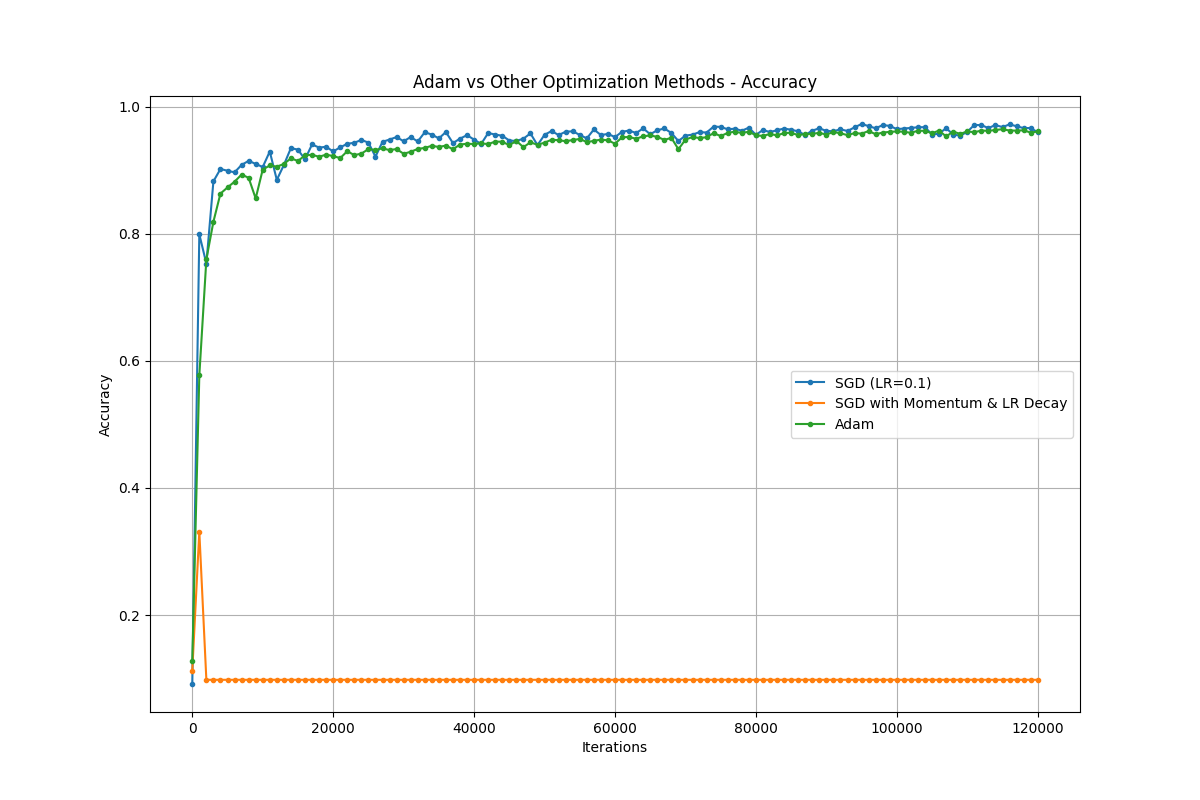
\includegraphics[width=1.1\textwidth]{plots/part3_adam_accuracy.png}
        \caption{Adam vs other optimization methods - accuracy.}
        \label{fig:adam_accuracy}
    \end{subfigure}
    \hfill
    %--- right plot ---------------------------------------------------
    \begin{subfigure}[t]{0.48\textwidth}
        \vspace{0pt}%  <-- ensures top alignment
        \centering
        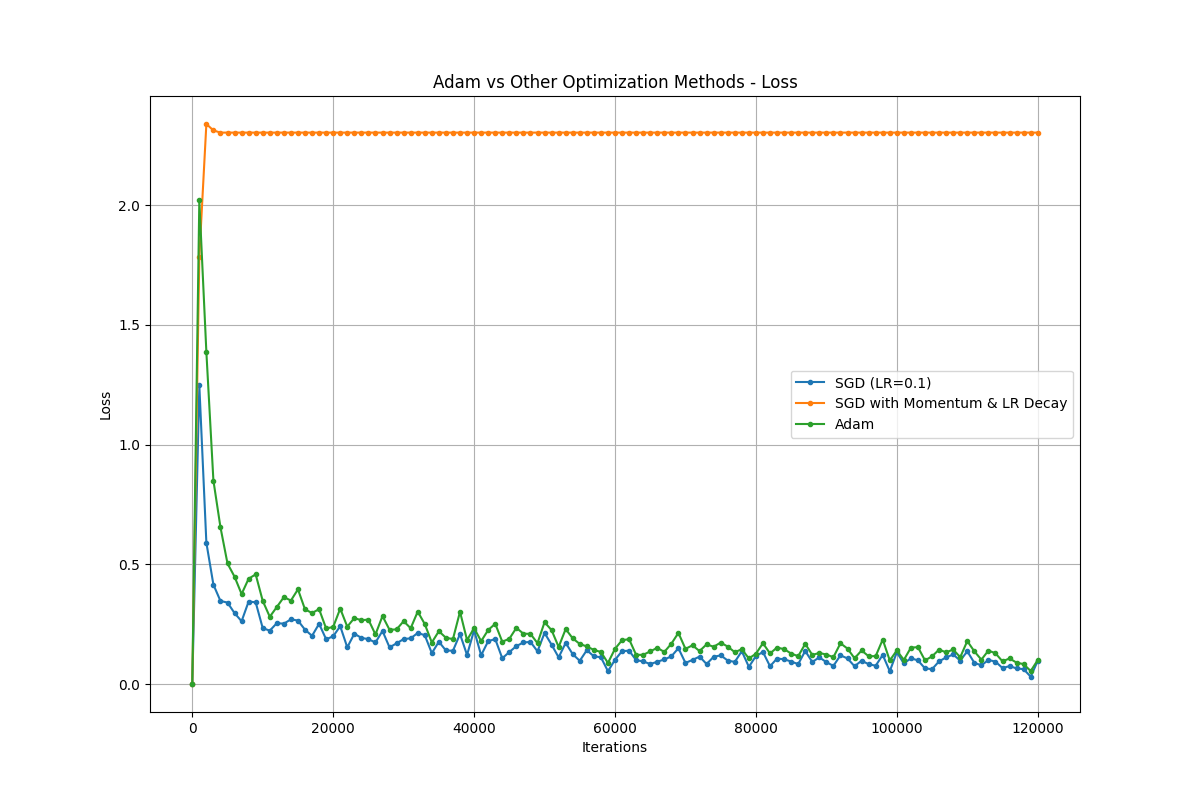
\includegraphics[width=1.1\textwidth]{plots/part3_adam_loss.png}
        \caption{Adam vs other optimization methods - loss.}
        \label{fig:adam_loss}
    \end{subfigure}
\end{figure}




It achieved a final accuracy of 96.11\%, which is competitive with the enhanced SGD methods.

The key strengths of Adam observed in the experiments were:
\begin{enumerate}
    \item \textbf{Parameter-specific adaptation}: Adam adapts learning rates individually for each parameter, allowing better handling of parameters with different gradient magnitudes.
    \item \textbf{Stability}: Adam showed more stable convergence with less hyperparameter tuning required compared to SGD variants.
    \item \textbf{Efficiency}: Adam achieved good results with a lower learning rate that would have been too slow for basic SGD.
\end{enumerate}

In this particular problem, SGD with learning rate decay outperformed Adam. This highlights that while adaptive methods like Adam are powerful general-purpose optimizers, problem-specific enhancements to simpler methods can sometimes yield better results.

\subsection{Optimal Hyperparameters and Comparison}

Comparing all techniques from Parts I-III, the optimal approach for this MNIST classification task was SGD with learning rate decay, with hyperparameters:
\begin{itemize}
    \item Initial learning rate: 0.1
    \item Final learning rate: 0.001
    \item Batch size: 10
\end{itemize}

This approach achieved the highest accuracy (97.45\%) and showed good convergence properties. Adam performed well (96.11\%) with minimal tuning, making it a good choice when extensive hyperparameter optimization is not feasible.

The comparison of all methods shows that:
\begin{enumerate}
    \item Basic SGD is effective but converges slowly in later stages
    \item Learning rate decay significantly improves final accuracy by allowing appropriate step sizes throughout training
    \item Momentum accelerates convergence, especially in areas with consistent gradient directions
    \item Combining momentum and learning rate decay can lead to instability if not carefully tuned
    \item Adam offers good performance with less tuning, making it practical for many applications
\end{enumerate}

These findings align with theoretical expectations about the strengths and weaknesses of each method and demonstrate how different optimization techniques can be applied to achieve superior performance, while highlighting the importance of stability considerations.

\section{Conclusion}

This report has explored various gradient-based optimization methods for training a neural network to classify MNIST handwritten digits. Starting with basic stochastic gradient descent, we progressively enhanced the algorithm with techniques such as learning rate decay and momentum, which significantly improved both convergence speed and final accuracy. We also implemented and evaluated the Adam optimizer, finding it to be competitive but slightly outperformed by our best SGD variant.

The highest accuracy achieved was 97.45\% using SGD with learning rate decay, demonstrating that even a relatively simple neural network architecture can achieve strong performance on the MNIST dataset when trained with appropriate optimization techniques.

The comparative analysis of different methods provides valuable insights into the trade-offs between optimization speed, stability, and final performance, which can guide the selection of appropriate algorithms for similar machine learning tasks. An important lesson from our experiments is that combining multiple enhancement techniques does not always yield better performance and can sometimes lead to instability if the interaction between techniques is not carefully managed.

\pagebreak

\begin{thebibliography}{9}

\bibitem{kingma2014adam}
Diederik P. Kingma and Jimmy Ba. Adam: A Method for Stochastic Optimization. \textit{arXiv}, 2014. arXiv:1412.6980.

\bibitem{lecun1998gradient}
Y. Lecun, L. Bottou, Y. Bengio, and P. Haffner. Gradient-based learning applied to document recognition. \textit{Proceedings of the IEEE}, 86(11):2278-2324, 1998.

\bibitem{bottou2008tradeoffs}
Léon Bottou and Olivier Bousquet. The tradeoffs of large scale learning. In \textit{Advances in Neural Information Processing Systems 20 (NIPS 2007)}, pages 161-168, 2008.

\end{thebibliography}

\end{document}
